\documentclass{beamer}
\usetheme{Luebeck}
\usepackage[utf8]{inputenc}
\usepackage[polish]{babel}
\usepackage[T1]{fontenc}
\usepackage[backend=bibtex]{biblatex}
\addbibresource{citations.bib}
\usepackage{hyperref}
\hypersetup{
colorlinks=True,
linkcolor=darkgray,
citecolor=red,
filecolor=olive,
urlcolor=purple}
\usepackage{minted}
\usepackage{float}
\usepackage{graphicx}
\usepackage{ulem}
\nocite{*}

\title{Fire and Smoke}
\author{Maciej Bartczak, Mikołaj Leonhardt, Wojciech Wiśniewski}
\date{Czerwiec 2023}

\begin{document}
\maketitle

\begin{frame}{Wstęp}
    Naszym zadaniem było zaimplementowanie trójwymiarowego automatu komórkowego służącego do symulacji rozprzestrzeniania się ognia oraz dymu. Implementacja została wykonana w języku C++ przy pomocy biblioteki graficznej OpenGL.
\end{frame}

\begin{frame}{Mechanizmy wykorzystane w modelu}
    Zaimplementowany przez nas model uwzględnia następujące mechanizmy:
    \begin{itemize}
        \item generowanie ciepła oraz dymu w procesie spalania
        \item kontaktowe przewodnictwo ciepła
        \item przewodnictwo ciepła poprzez konwekcje
        \item rozprzestrzenianie się ognia
        \item rozprzestrzenianie się dymu
    \end{itemize}

\end{frame}

\begin{frame}{Zastosowane sąsiedztwo}
    W celu uproszczenia modelu i ułatwienia obliczeń, podobnie jak w innych badaniach tego typu, zastosowano sąsiedztwo oparte o relację przylegania do siebie sześcianów. Oznacza to, że w naszej trójwymiarowej przestrzeni automatu komórkowego, każda komórka wchodzi w interakcje z sześcioma najbliższymi jej komórkami, które są jej bezpośrednio przyległe wzdłuż osi X, Y, Z (góra, dół, lewo, prawo, przód, tył). Jest to trójwymiarowy odpowiednik sąsiedztwa Moore'a.
\end{frame}

\begin{frame}{Własności zastosowanych materiałów}
    \begin{table}[]
        \footnotesize
        \begin{tabular}{llllll}
        & Powietrze & Beton & Drewno & Dywan & Materiał \\
        Palność & Nie & Nie & Tak & Tak & Tak \\
        Gęstość [\(\frac{kg}{m^3}\)] & 1.29 & 2200 & 400 & 300 & 400 \\
        Ciepło właściwe [\(\frac{J}{kg \cdot K}\)] & 1005 & 900 & 2390 & 5200 & 2390 \\
        Wsp. przewodnictwa & 0.026 & 0.005 & 0.3 & 0.174 & 0.3 \\
        T. zapłonu [\(\circ C\)] & - & - & 250 & 120 & 350\\
        T. samozapłonu [\(\circ C\)] & - & - & 2000 & 750 & 1400 \\
        Czas palenia [\(s\)] & - & - & 20 & 15 & 20 \\
        Wsp. em. ciepła [\(\frac{J}{s}\)] & - & - & 1500 & 500 & 1500 \\
        Wsp. em. dymu & - & - & 0.3 & 0.8 & 1 \\
        \end{tabular}
    \end{table}

    Powyższe dane zostały zaczerpnięte z pracy [1].
\end{frame}

\begin{frame}{Generowanie ciepła}
    Ciepło jest generowane przez palące się komórki korzystając z fizycznych własności zastosowanych materiałów.
    \newline

    Ciepło wygenerowane przez płonący materiał o współczynniku emisji ciepła \(P \left[\frac{J}{s}\right]\) jest dane wzorem:
    \begin{equation}
        Q = P \cdot t
    \end{equation}

    Zmianę temperatury komórki (o cieple właściwym \(c\) i masie \(m\)) można policzyć według wzoru:
    \begin{equation}
        T_{t+1} = T_t + \frac{Q}{m \cdot c}
    \end{equation}
\end{frame}

\begin{frame}{Przewodnictwo ciepła}
    Przewodnictwo ciepła to proces, w którym energia termiczna jest przenoszona wewnątrz ciała lub między ciałami w bezpośrednim kontakcie, poprzez drgania cząstek. W naszym modelu, przewodnictwo ciepła jest symulowane poprzez bezpośrednią interakcję między sąsiadującymi komórkami.
    \newline

    Korzystając z następujących oznaczeń:
    \begin{itemize}
        \item \(N(c)\) to sąsiedztwo komórki \(c\)
        \item \(\lambda(c)\) to współczynnik przewodnictwa komórki \(c\)
    \end{itemize}
    Można policzyć zmianę temperatury rozważanej komórki:
    \begin{equation}
        T_{t+1}(c) = T_t(c) + \sum_{c' \in N(c)} \lambda(c') \cdot \left(T_t(c) - T_t(c')\right)
    \end{equation}
\end{frame}

\begin{frame}{Konwekcja}
    W naszym automacie konwekcja jest symulowana przez ruch ciepła w górę poprzez komórki powietrza.
    \newline

    Korzystając z oznaczeń:
    \begin{itemize}
        \item \(c_U\) - górna komórka
        \item \(c_L\) - dolna komórka
        \item \(\alpha\) - współczynnik konwekcji
    \end{itemize}
    Można policzyć zmianę temperatury rozważanych komórek:
    \begin{equation}
        \begin{array}{l}
            T_{t+1}(c_U) = T_t(c_U) + \alpha \cdot \left( T_t(c_U) - T_t(c_L) \right) \\
            T_{t+1}(c_L) = T_t(c_L) - \alpha \cdot \left( T_t(c_U) - T_t(c_L) \right)
        \end{array}
    \end{equation}
\end{frame}

\begin{frame}{Rozprzestrzenianie się ognia}
    Dla każdego zastosowanego materiału zostały zdefiniowane temperatury zapłonu oraz samozapłonu.
    \newline

    Pozwala nam to zdefiniować dwa warunki wystarczające do zapalenia się komórki:
    \begin{enumerate}
        \item Temperatura rozważanej komórki jest wystarczająca oraz istnieje sąsiad, który palił się wystarczająco długo:
        \begin{equation}
            \exists c' \in N(c): T(c) \geq T_z(c) \wedge t(c') \geq t_z(c')
        \end{equation}

        \item Temperatura rozważanej komórki przekroczyła temperaturę samozapłonu:
            \begin{equation}
                T(c) \geq T_s(c)
            \end{equation}
    \end{enumerate}
\end{frame}

\begin{frame}{Rozprzestrzenianie się dymu}
    Rozważając komórkę naszego automatu komórkowego, w sytuacji, gdy dostępna pojemność na dym w komórce stanowi \(10\%\) lub mniej całościowej pojemności, dystrybucja dymu jest realizowana pomiędzy pięcioma komórkami sąsiednimi, pomijając komórkę bezpośrednio powyżej.

    Dla każdej z pięciu komórek, obecna komórka przekazuje najwyżej 1/6 swojego dymu, pod warunkiem, że komórka docelowa jest w stanie go pomieścić. Równocześnie, obecna komórka może przyjąć dym od każdej z pięciu komórek, jednak najwyżej 1/6 ilości dymu każdej z nich, i tylko w granicach swojej dostępnej pojemności.

    Gdy dostępna pojemność na dym w komórce przekracza \(10\%\) jej całościowej pojemności, dystrybucja dymu jest analogiczna, ale uwzględnia wszystkie sześć komórek sąsiadujących.
\end{frame}

\begin{frame}{Problemy związane z radiacją}
    Radiacja to proces przekazywania energii cieplej za pomocą fal elektromagnetycznych, bez bezpośredniego kontaktu. Implementacja tego procesu w modelu automatu komórkowego stanowi duże wyzwanie, ponieważ nie jest ona ograniczona do bezpośrednich sąsiadów.
    \newline

    Natężenie promieniowania maleje odwrotnie proporcjonalnie do kwadratu odległości między komórkami.
    Powoduje to konieczność zbudowania oraz utrzymywania sąsiedztwa według relacji wzajemnej widoczności każdej pary komórek, co jest problemem trudnym obliczeniowo. Taka naiwna implementacja nie uwzględniałaby także obliczeń wynikających z różnych kątów padania promieniowania. Z wyżej wymienionych powodów zaniechaliśmy implementacji Radiacji.
\end{frame}

\begin{frame}{Problemy z powstawaniem słupów ognia}
    Przy próbie symulacji słupów ognia w automacie komórkowym napotkaliśmy wiele wyzwań. W szczególności, dynamika płomienia obejmuje skomplikowane interakcje między gazami, temperaturą i ciśnieniem, które są trudne do modelowania w ramach prostych reguł automatu komórkowego.

    Ze względu na te wyzwania, podjęliśmy decyzję o wprowadzeniu uproszczeń. Zamiast próbować symulować cały słupek ognia, skupiliśmy się na modelowaniu palenia się pojedynczych komórek.
\end{frame}

\begin{frame}{Przykłady rzeczywistych pożarów}
\begin{figure}[htbp]
  \centering
  \begin{minipage}{.45\textwidth}
    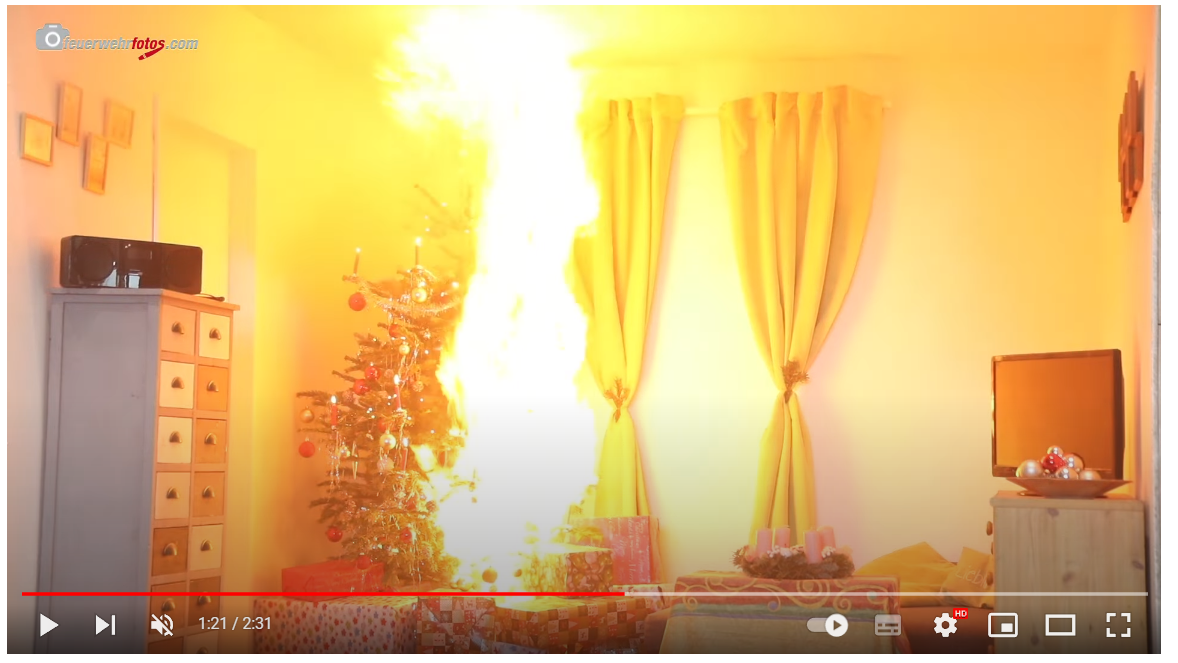
\includegraphics[width=\textwidth]{1.png}
    \caption{Przykład 1 - pożar drzewka choinkowego}
    \label{fig:image1}
  \end{minipage}%
  \hfill
  \begin{minipage}{.45\textwidth}
    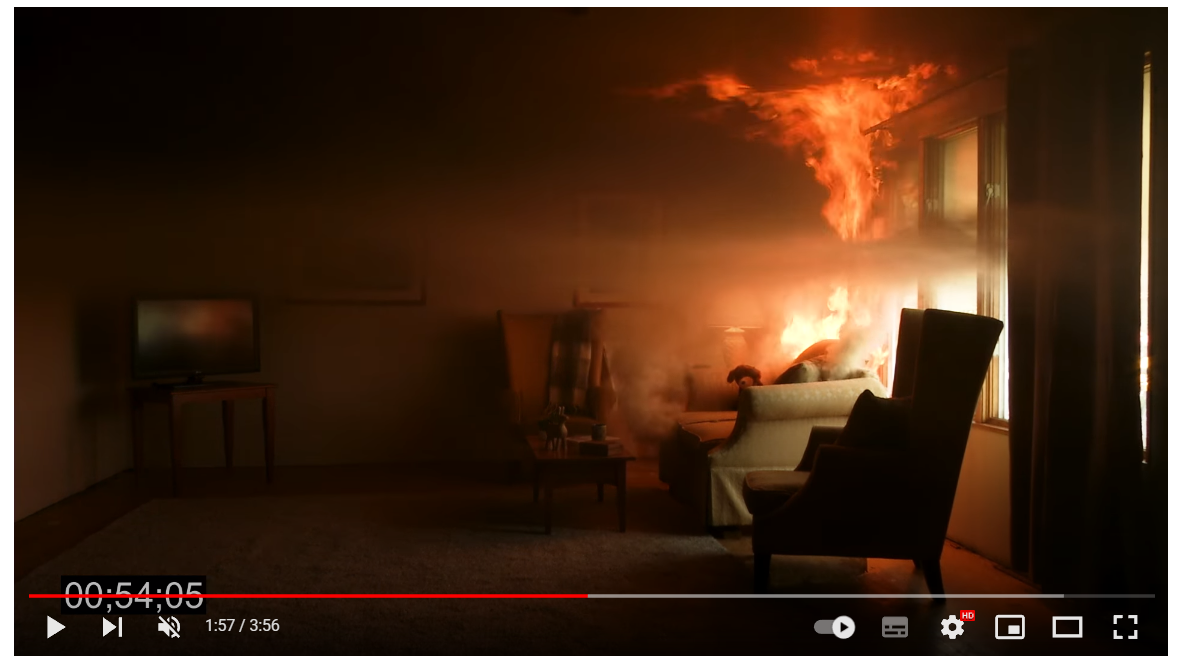
\includegraphics[width=\textwidth]{2.png}
    \caption{Przykład 2 - pożar kanapy}
    \label{fig:image2}
  \end{minipage}
\end{figure}

Na obu powyższych przykładach można zaobserwować zjawiska powstawania słupów ognia oraz radiacji, których nie udało nam się zaimplementować.
\end{frame}

\begin{frame}{Nasza symulacja - dym oraz ogień}
\begin{figure}[htbp]
  \centering
  \begin{minipage}{.45\textwidth}
    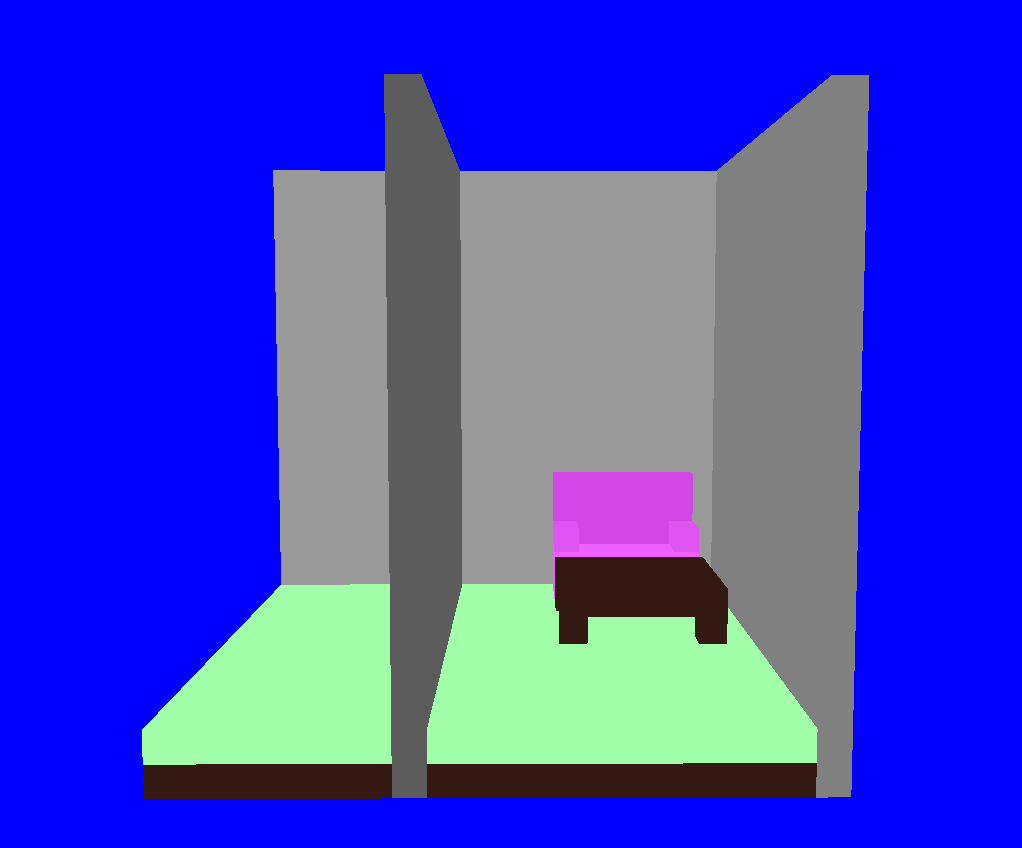
\includegraphics[width=\textwidth]{3.png}
    \caption{Scena przed pożarem}
    \label{fig:image3}
  \end{minipage}%
  \hfill
  \begin{minipage}{.45\textwidth}
    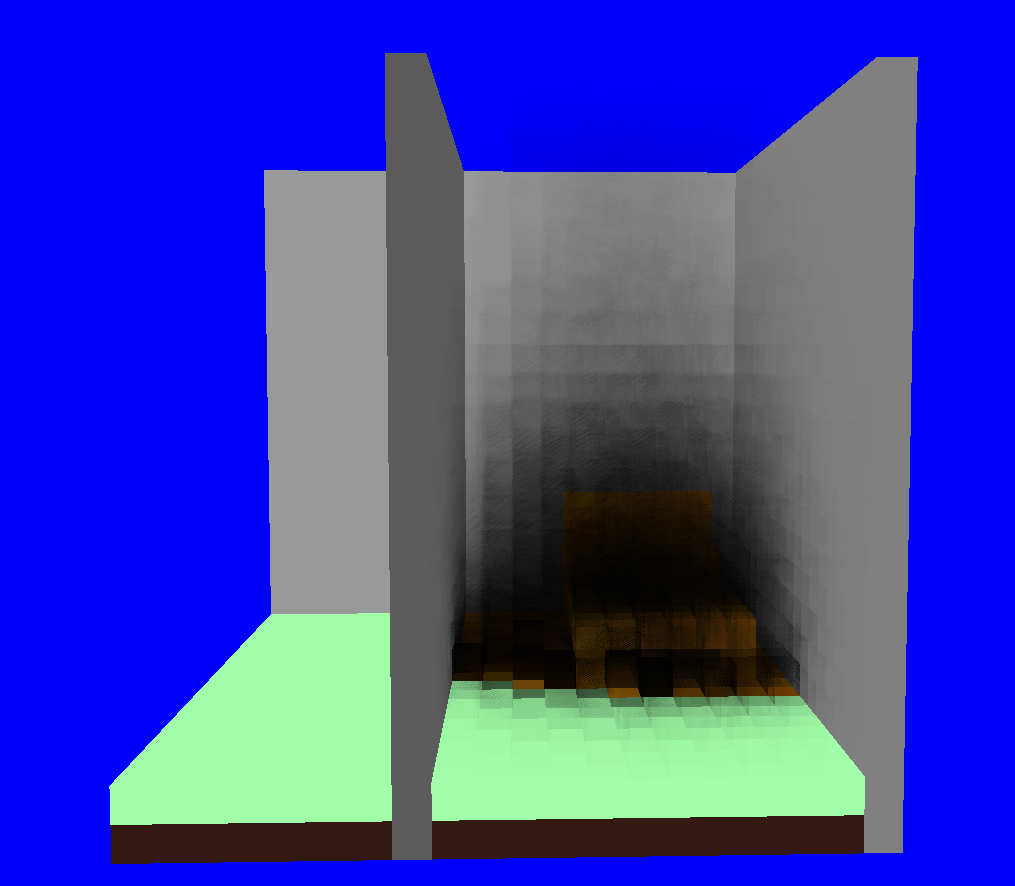
\includegraphics[width=\textwidth]{4.png}
    \caption{Scena w trakcie pożaru}
    \label{fig:image4}
  \end{minipage}
\end{figure}

Można zauważyć rozprzestrzenianie się ognia (pomarańczowe bloki) oraz dymu.
\end{frame}

\begin{frame}{Nasza symulacja - temperatura}
\begin{figure}[htbp]
  \centering
  \begin{minipage}{.45\textwidth}
    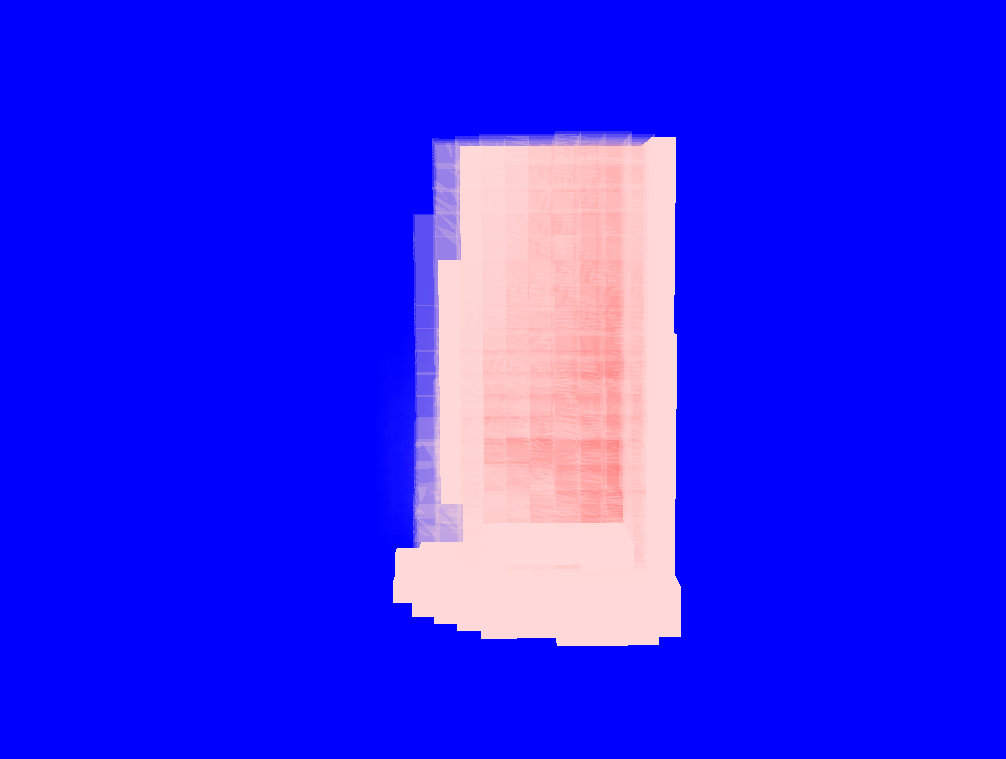
\includegraphics[width=\textwidth]{5.png}
    \caption{Początkowe stadium pożaru}
    \label{fig:image5}
  \end{minipage}%
  \hfill
  \begin{minipage}{.4\textwidth}
    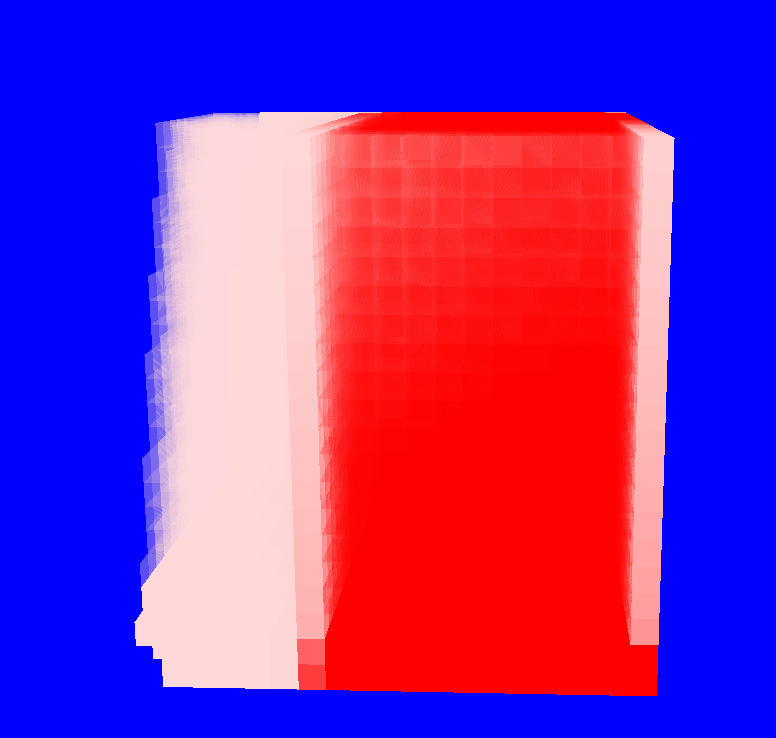
\includegraphics[width=\textwidth]{6.png}
    \caption{Zaawansowane stadium pożaru}
    \label{fig:image6}
  \end{minipage}
\end{figure}

Można zauważyć, że temperatura jest największa w miejscu wybuchu ognia (dolna część kanapy). Ciepło wypełnia pokój i poprzez przewodnictwo dociera do sąsiedniego pokoju.
\end{frame}

\begin{frame}{Wnioski}
    Nasza próba implementacji tej symulacji pozwoliła nam poznać wyzwania wynikające z takiego zadania. Obliczenia trójwymiarowe są wymagające obliczeniowo, a ich implementacja na karcie graficznej wymaga głębokiego zrozumienia OpenGL. Mimo intensywnych starań nie udało nam się w pełni przenieść wszystkich niezbędnych obliczeń na GPU, co przekładało się na problemy z wydajnością. Byliśmy zmuszeni dokonać pewnych uproszczeń w naszych mechanikach symulacyjnych, co jest bezpośrednią konsekwencją tych trudności. Nie pomniejsza to jednak wartości doświadczenia, które zdobyliśmy w trakcie tej próby, i stanowi cenne lekcje na przyszłość.
\end{frame}

\begin{frame}{Referencje}
    \begin{enumerate}
        \item Wąs, J., Karp, A., Łukasik, S., Pałka, D. (2020). Modeling of Fire Spread Including Different Heat Transfer Mechanisms Using Cellular Automata. In: , et al. Computational Science – ICCS 2020. ICCS 2020. Lecture Notes in Computer Science(), vol 12137. Springer, Cham. \url{https://doi.org/10.1007/978-3-030-50371-0_33}
        \item M. Byari, A. Bernoussi, O. Jellouli, M. Ouardouz, M. Amharref, Multi-scale 3D cellular automata modeling: Application to wildland fire spread, Chaos, Solitons \& Fractals, Volume 164, 2022, 112653, ISSN 0960-0779, \url{https://doi.org/10.1016/j.chaos.2022.112653}
        \item Brennender Christbaum / Weihnachtsbaum \url{https://www.youtube.com/watch?v=YDCwJhCoN9c}
        \item Living room fires with and without a fire sprinkler (Timecode) \url{https://www.youtube.com/watch?v=EehF0UHYaYk}
    \end{enumerate}
\end{frame}

\end{document}
